\documentclass[14pt, a4paper]{extarticle}

\usepackage{my_GOST}
\usepackage{hyperref}
\usepackage{listings}
\usepackage{array}
\usepackage{caption}
\hypersetup{
	pdftex,
	colorlinks = true,
	linkcolor = black,
	filecolor = magenta,
	citecolor = green,      
	urlcolor = cyan,
}

% к таблице и листингу подпись сверху, перед каждым иллюстративным материалом анонсировать
% написатьт в квадратных скобках к рекурсии комментарием что это метод и понятно почему вызываем его снова
\definecolor{mylightgray}{RGB}{240,240,240}
\definecolor{mygreen}{rgb}{0,0.6,0}
\definecolor{mygray}{rgb}{0.5,0.5,0.5}
\definecolor{mymauve}{rgb}{0.58,0,0.82}

\lstset{
	backgroundcolor=\color{mylightgray},rulecolor=\color{red},  % choose the background color; you must add \usepackage{color} or \usepackage{xcolor}; should come as last argument
	basicstyle=\footnotesize\ttfamily,        % the size of the fonts that are used for the code
	breakatwhitespace=false,         % sets if automatic breaks should only happen at whitespace
	breaklines=true,                 % sets automatic line breaking
	captionpos=t,                    % sets the caption-position to bottom
	commentstyle=\color{mygreen},    % comment style
	extendedchars=false,              % lets you use non-ASCII characters; for 8-bits encodings only, does not work with UTF-8
	firstnumber=0,                % start line enumeration with line 1000
	frame=shadowbox,
	%rulesepcolor=\color{green},	                   % adds a frame around the code
	keepspaces=true,                 % keeps spaces in text, useful for keeping indentation of code (possibly needs columns=flexible)
	keywordstyle=\color{blue}\textbf,       % keyword style
	language=C++,                 % the language of the code
	morekeywords={*,...},            % if you want to add more keywords to the set
	numbers=left,                    % where to put the line-numbers; possible values are (none, left, right)
	numbersep=5pt,                   % how far the line-numbers are from the code
	numberstyle=\scriptsize\color{mygray}, % the style that is used for the line-numbers
	rulecolor=\color{black},         % if not set, the frame-color may be changed on line-breaks within not-black text (e.g. comments (green here))
	showspaces=false,                % show spaces everywhere adding particular underscores; it overrides 'showstringspaces'
	showstringspaces=false,          % underline spaces within strings only
	showtabs=false,                  % show tabs within strings adding particular underscores
	stepnumber=1,                    % the step between two line-numbers. If it's 1, each line will be numbered
	stringstyle=\color{mymauve},     % string literal style
	tabsize=4,	                   % sets default tabsize to 2 spaces
	title=\lstname                   % show the filename of files included with \lstinputlisting; also try caption instead of title
}
\usepackage{YATPR}

\usepackage{float}

\begin{document}
\begin{titlepage}
	\newgeometry{pdftex, left=2cm, right=2cm, top=2.5cm, bottom=2.5cm}
	\fontsize{12pt}{12pt}\selectfont
	\noindent \begin{minipage}{0.15\textwidth}
		
\includegraphics[width=\linewidth]{pictures/b_logo.jpg}
	\end{minipage}
	\noindent\begin{minipage}{0.9\textwidth}\centering
		\textbf{Министерство науки и высшего образования Российской Федерации}\\
		\textbf{Федеральное государственное бюджетное образовательное учреждение высшего образования}\\
		\textbf{«Московский государственный технический университет имени Н.Э.~Баумана}\\
		\textbf{(национальный исследовательский университет)»}\\
		\textbf{(МГТУ им. Н.Э.~Баумана)}
	\end{minipage}
	
	\noindent\rule{18cm}{3pt}
	\newline\newline
	\noindent ФАКУЛЬТЕТ $\underline{\text{«Информатика и системы управления»}}$ \newline\newline
	\noindent КАФЕДРА $\underline{\text{«Программное обеспечение ЭВМ и информационные технологии»}}$\newline\newline\newline\newline\newline\newline\newline
	
	
	\begin{center}
		\Large\textbf{Отчет по лабораторной работе №5}\newline
	\end{center}
	
	\noindent\textbf{Название} $\underline{\text{~Моделирование работы информационного центра~~~~~~~~~}}$\newline\newline\newline
	\noindent\textbf{Дисциплина} $\underline{\text{~Моделирование~~~~~~~~}}$\newline\newline
	\noindent\textbf{Студент} $\underline{\text{Зайцева А. А.~~~~~~~~~~~~~~~~~~~~~~~~~~~~~~~~~~~~~~~~~}}$\newline\newline
	\noindent\textbf{Группа} $\underline{\text{ИУ7-72Б~~~~~~~~~~~~~~~~~~~~~~~~~~~~~~~~~~~~~~~~~~~~}}$\newline\newline
	\noindent\textbf{Оценка (баллы)} $\underline{\text{~~~~~~~~~~~~~~~~~~~~~~~~~~~~~~~~~~~~~~~~~~~~~~~~~}}$\newline\newline
	\noindent\textbf{Преподаватель}$\underline{\text{~Рудаков И. В.~~~~~~~~~~}}$\newline
	
	\begin{center}
		\vfill
		Москва~---~\the\year
		~г.
	\end{center}
 \restoregeometry
\end{titlepage}


\setcounter{page}{2}

\section{Задание}
Написать программу, которая позволяет определить время пребывания сложной системы в каждом из состояний в установившемся режиме работы. Количество состояний $\le 10$.

Реализовать интерфейс, который позволяет указать количество состояний и значения матрицы вероятностей переходов, а также отображает результаты работы программы: графики вероятностей состояний, время стабилизации вероятности каждого состояния, стабилизировавшееся значение вероятности каждого состояния.

\section{Теоретические сведения}

Случайный процесс, протекающий в некоторой системе S, называется Марковским, если он обладает следующим свойством: для каждого момента времени вероятность любого состояния системы в будущем зависит только от её состояния в настоящем и не зависит от того, когда и каким образом она пришла в это состояние (то есть не зависит от прошлого).

Для марковского процесса обычно составляются уравнения Колмогорова: 
\begin{equation*}
	F = (P'(t), P(t), \lambda) = 0,
\end{equation*}где $\lambda$ - некоторый набор коэффициентов.

Интегрирование системы уравнений даёт искомые вероятности как функции времени. Начальное условие берется в зависимости от того, какое было начальное состояние системы. Кроме того, необходимо добавить условие нормировки: $\sum^{n}_{i=1}{P_i}(t) = 1$ для любого момента t. $P_i(t)$ -- вероятность того, что в момент t система будет находиться в i-м состоянии.

Уравнения Колмогорова строятся по следующим правилам:
\begin{itemize}
	\item В левой части каждого уравнения стоит производная вероятности i-ого состояния, а правая часть содержит столько членов, сколько переходов связано с данным состоянием. 
	
	\item Если переход осуществляется из этого состояния, то соответствующий член имеет знак минус, если в это состояние, то плюс. 
	
	\item Каждый член равен произведению плотности вероятности перехода (интенсивности), соответствующей данному переходу, и вероятности того состояния, из которого осуществляется переход.
\end{itemize}


Для определения предельных вероятностей при $t \to \infty$ (то есть вероятностей в стационарном режиме работы), необходимо приравнять левые части уравнений (то есть производные) к нулю и решить полученную систему линейных уравнений. 

Чтобы найти время стабилизации, необходимо найти найти момент времени $t_s$, когда значение производной $P_{i}^{'}(t_s)$ меньше заранее заданного $\varepsilon$. Тогда приращение соответствующей вероятности к следующему моменту времени $\Delta P_{i} = P_{i}^{'}(t_s)\Delta t$ будет меньше некоторой погрешности.

%времени пребывания системы в каждом состоянии
%Для нахождения времен стабилизации, необходимо с интервалом $\Delta t$ находить каждую вероятность в каждый момент времени, вычисляя приращения для каждой вероятности $\Delta P_{i} = P_{i}^{'}(t) * \Delta t$. Эти вычисления необходимо продолжать, пока разница между предыдущей и текущей вероятностью больше заранее заданного $\epsilon$.




\section{Результаты работы программы}
%Условием стабилизации вероятности состояния $i$ принимается величина $P_i(t_{stab})$, где $t_{stab}$ - наименьшее время, при котором ${P'}_i(t_{stab}) < 10^{-7}$. 

В начале работы система находится в первом состоянии, $\varepsilon$ для определения стабилизации вероятности принимается равным $10^{-5}$.



\newpage
На рисунке \ref{pic:1} приведен пример работы программы для 3 состояний.
\begin{figure}[h]
	\begin{center}
		{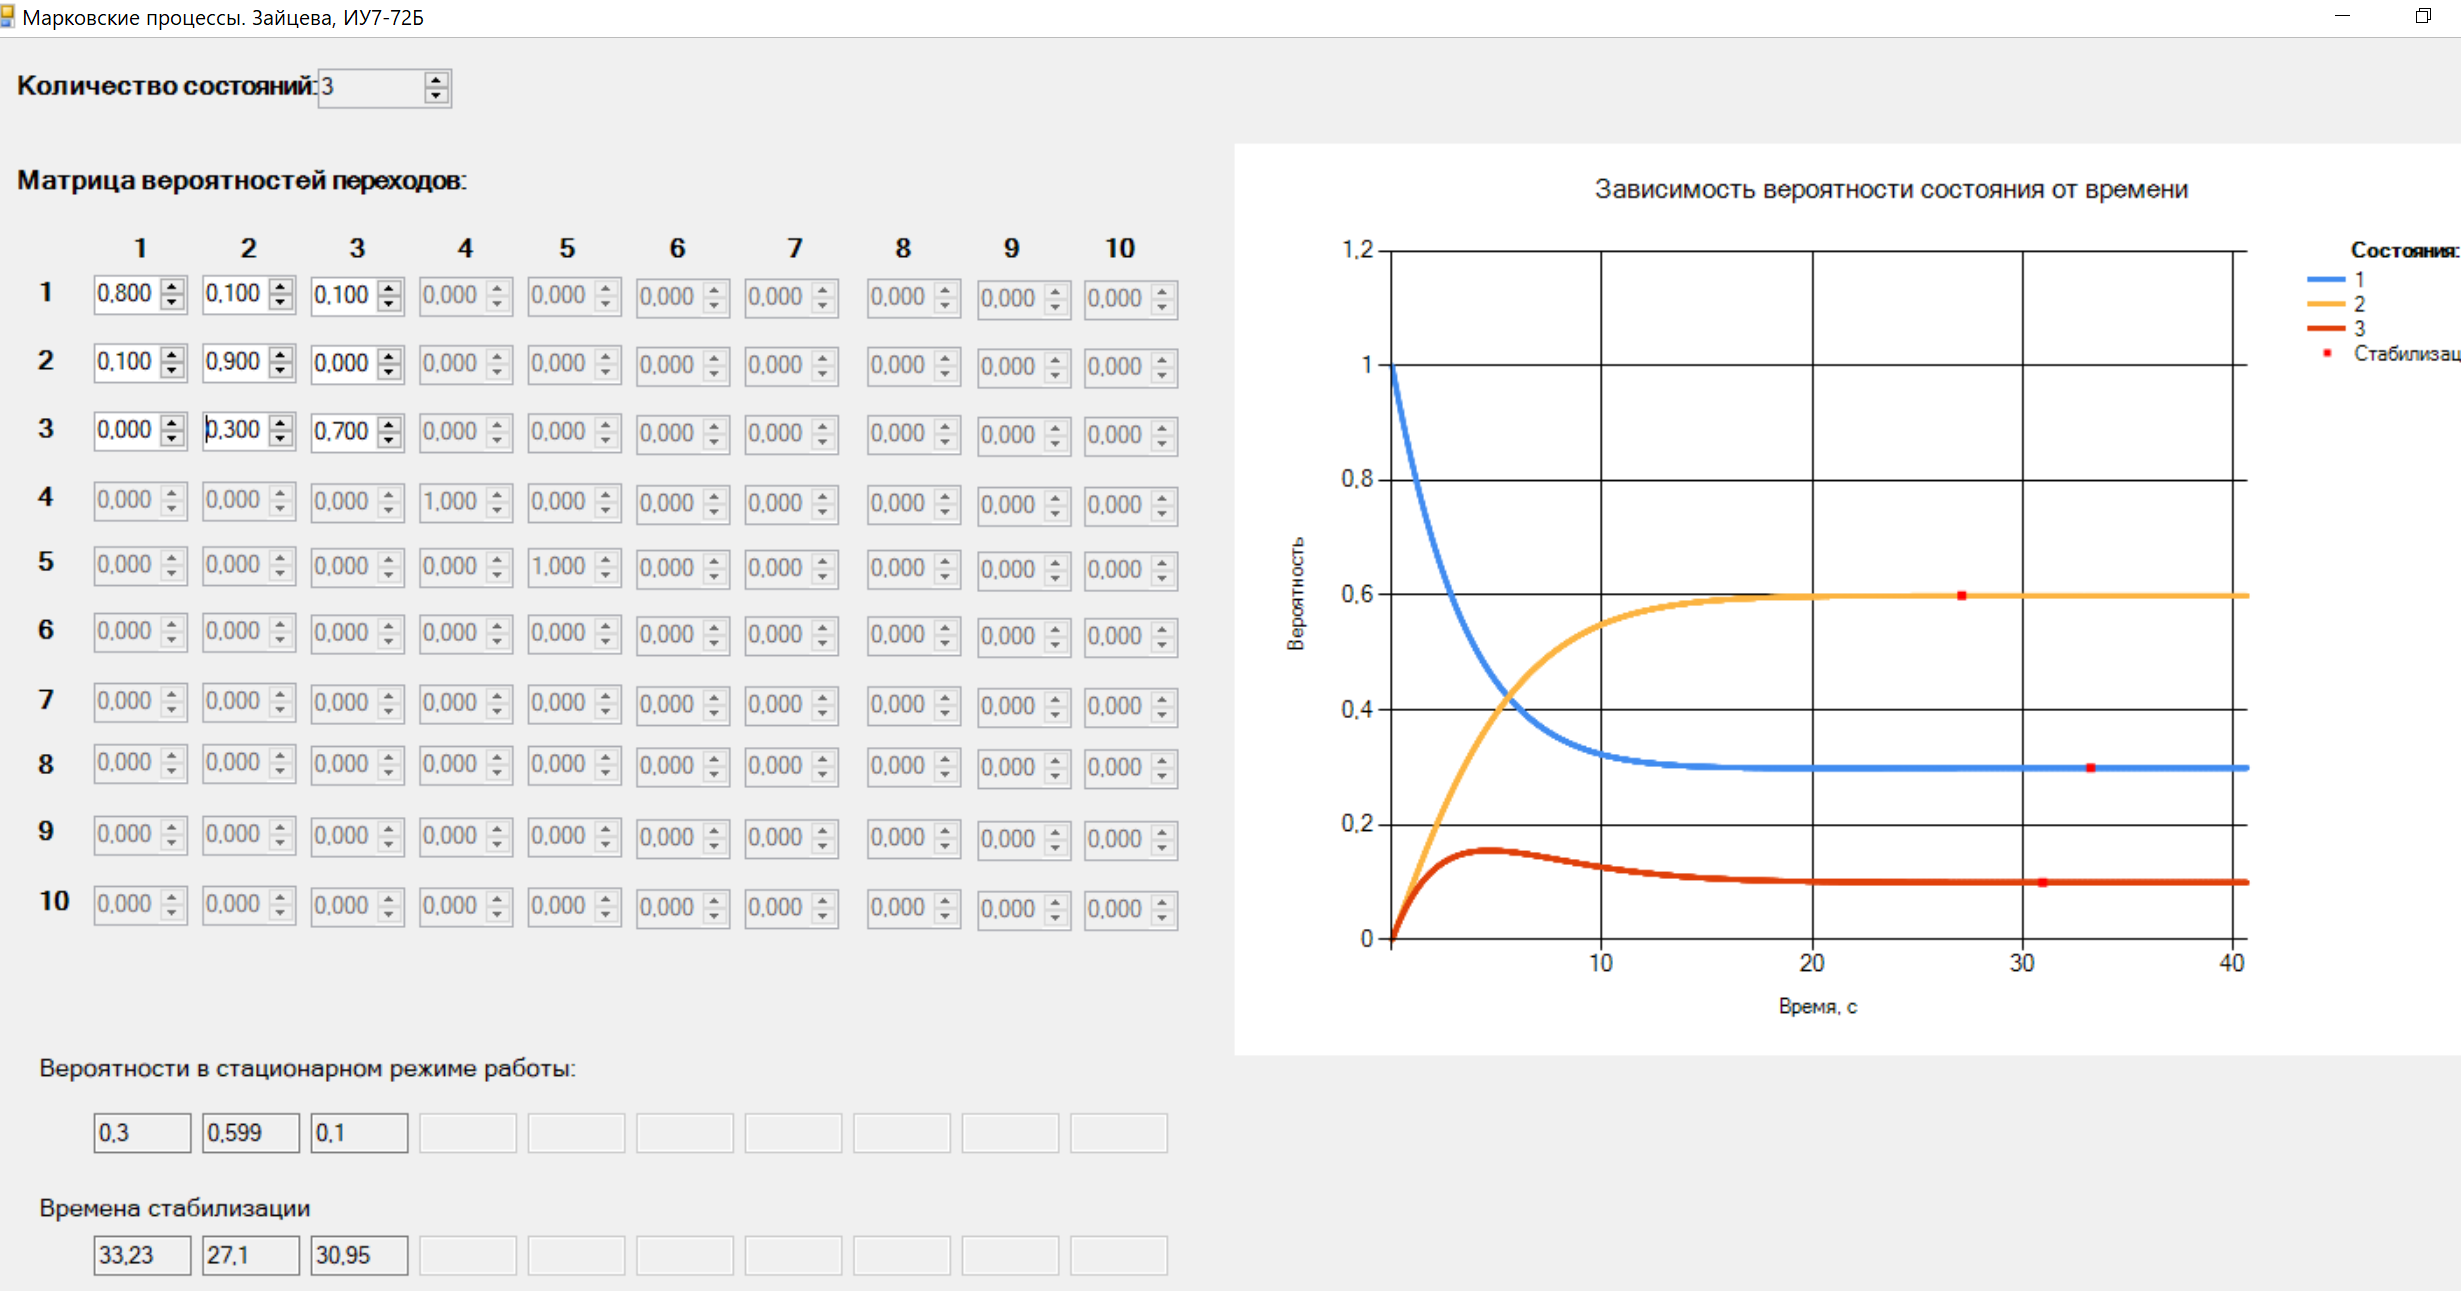
\includegraphics[scale=0.45]{pictures/1.png}
			\caption{Пример работы программы для 3 состояний}
			\label{pic:1}}
	\end{center}
\end{figure}

Проверим результаты, приведенные на рисунке выше. Составим систему линейных уравнений для определения вероятностей в стационарном режиме: составим уравнения Колмогорова и приравняем левые части к 0, а также добавим условие нормировки.
\begin{equation}
	\left\{\begin{array}{l}
		0 = 0.1 \cdot P_2 - 0.1 \cdot P_1 - 0.1 \cdot P_1 \\
		0 = 0.1 \cdot P_1 + 0.3 \cdot P_3 - 0.1 \cdot P2 \\
		0 = 0.1 \cdot P_1 - 0.3 \cdot P_3 \\
		P_1 + P_2 + P_3 = 1
	\end{array}\right.
\end{equation}

\begin{equation}
	\left\{\begin{array}{l}
		P_1 = \frac{3}{10} \\
		P_2 = 2 \cdot P_1 = \frac{6}{10} \\
		P_3 = \frac{1}{3} \cdot P_1 = \frac{1}{10} \\
	\end{array}\right.
\end{equation}

Вычисленные значения совпадают с результатами программы.



\newpage
На рисунке \ref{pic:2} вероятность перехода из второго состояния в любое другое равна 0, поэтому в стабилизировавшемся режиме вероятность этого состояния примерно равна 1, а остальных -- 0.
\begin{figure}[h]
	\begin{center}
		{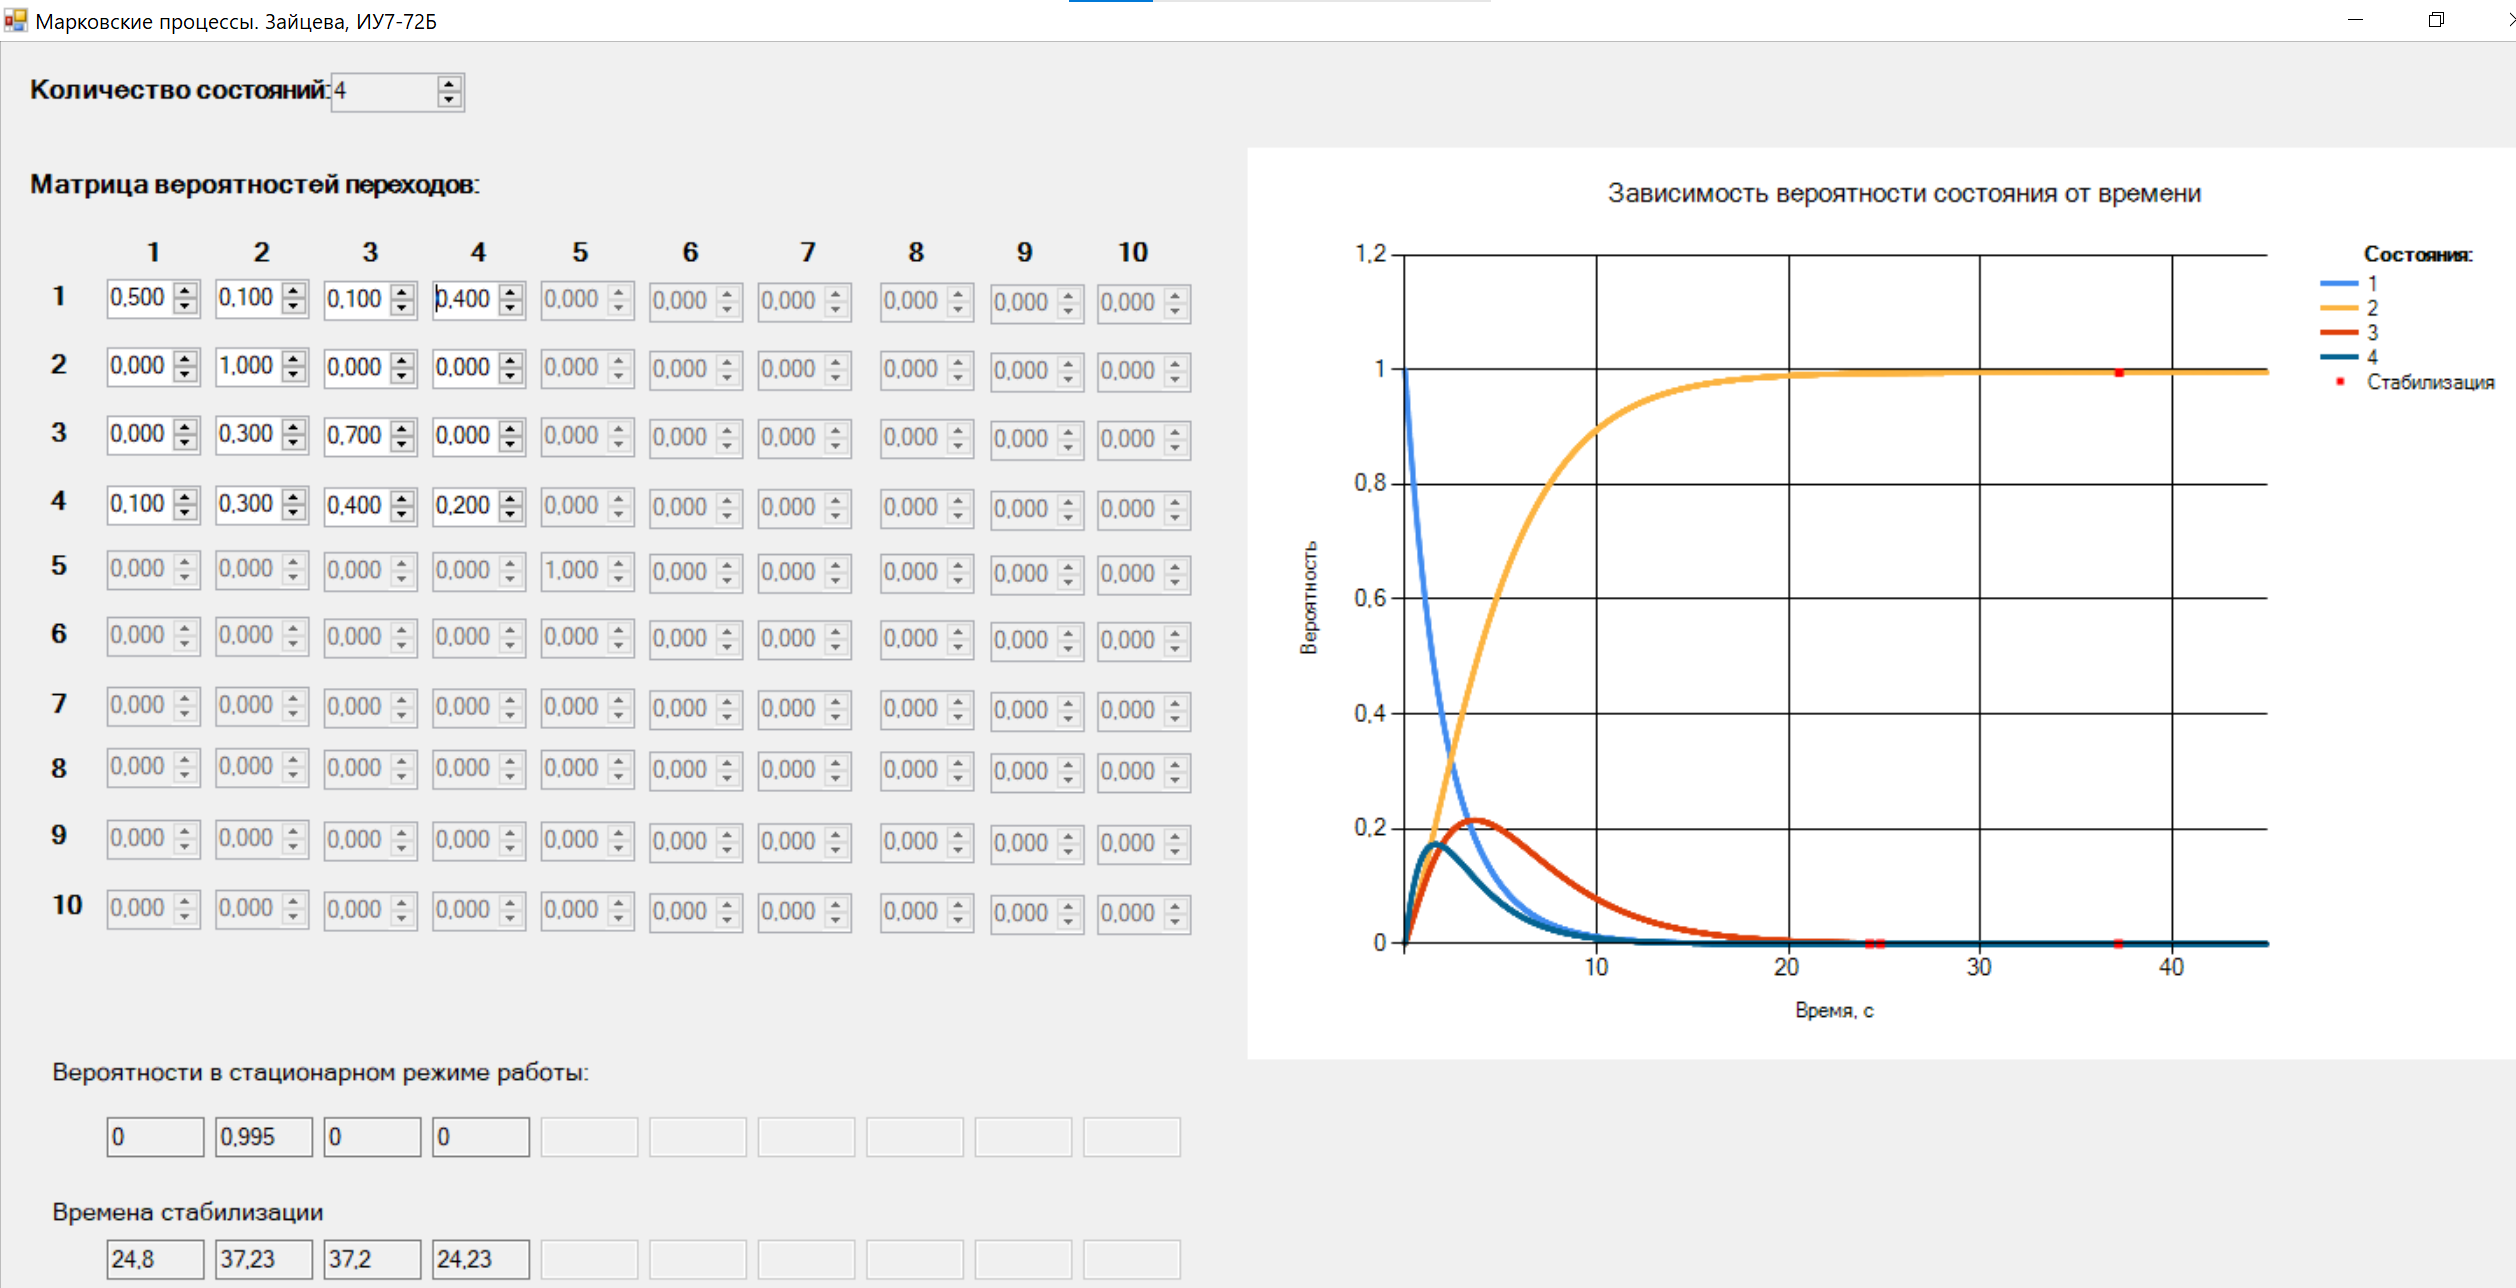
\includegraphics[scale=0.45]{pictures/2.png}
			\caption{Пример работы программы для 4 состояний}
			\label{pic:2}}
	\end{center}
\end{figure}


\newpage
На рисунке \ref{pic:3} из первого состояния есть вероятность перейти в другие, но вероятность попасть из любого состояния в первое равна 0, поэтому и в стабилизировавшемся режиме вероятность первого состояния равна 0.
\begin{figure}[h]
	\begin{center}
		{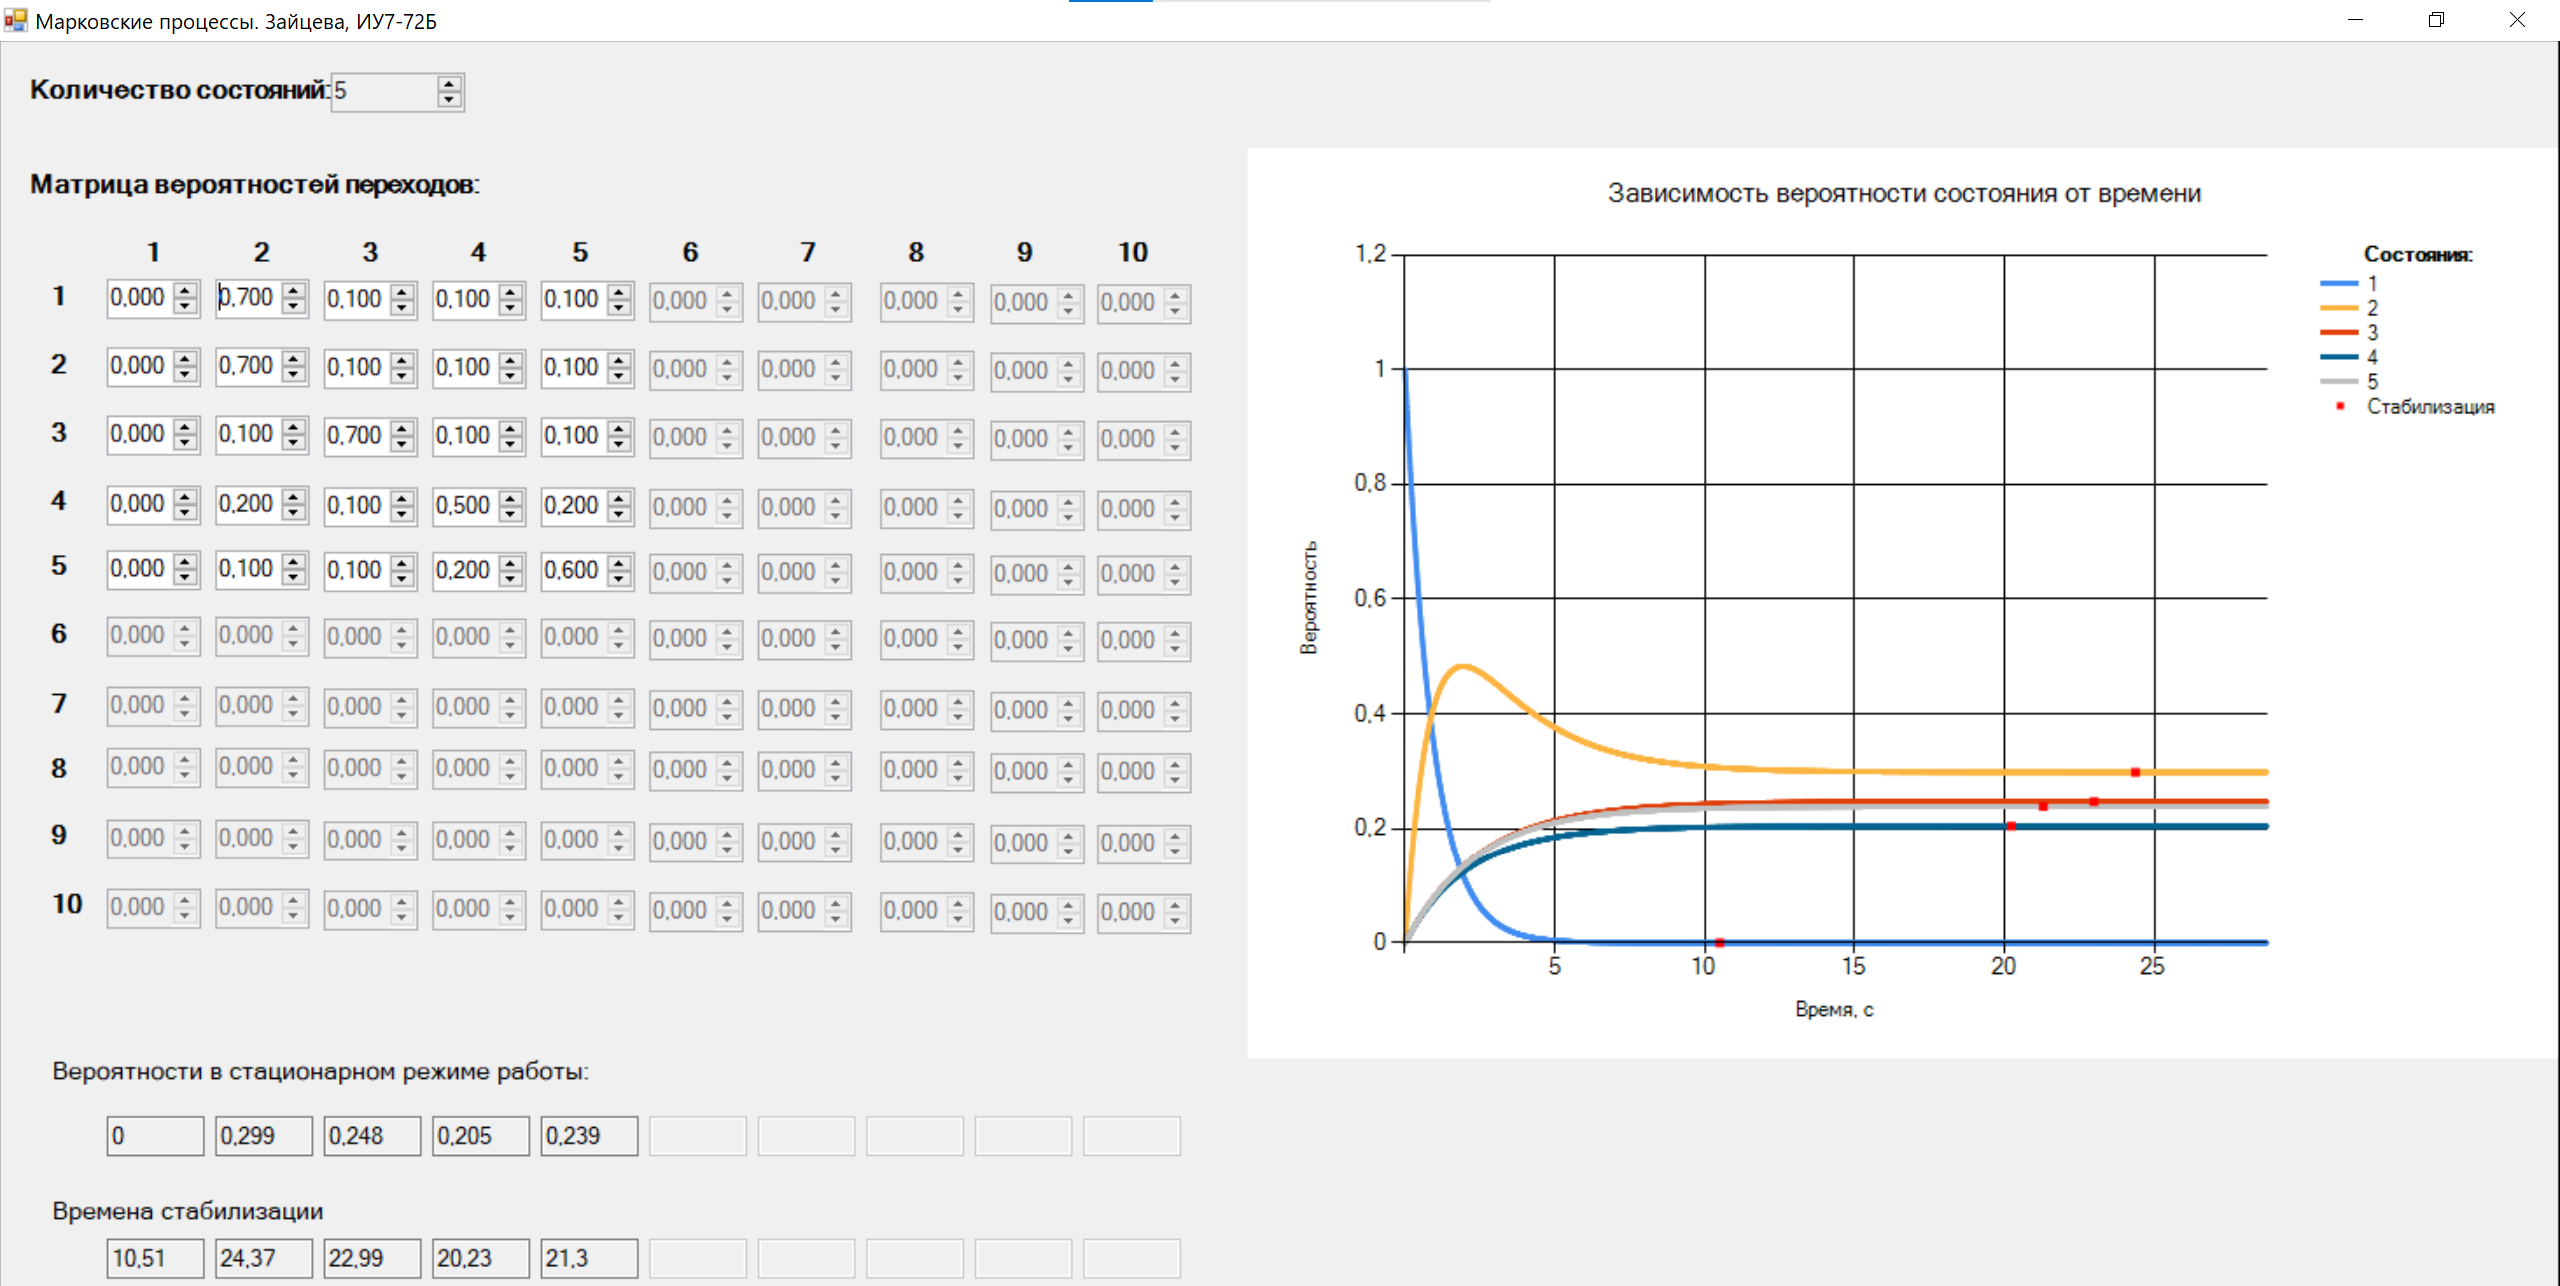
\includegraphics[scale=0.45]{pictures/3.png}
			\caption{Пример работы программы для 5 состояний}
			\label{pic:3}}
	\end{center}
\end{figure}

\newpage
На рисунке \ref{pic:4} приведен пример работы программы для 10 состояний.
\begin{figure}[h]
	\begin{center}
		{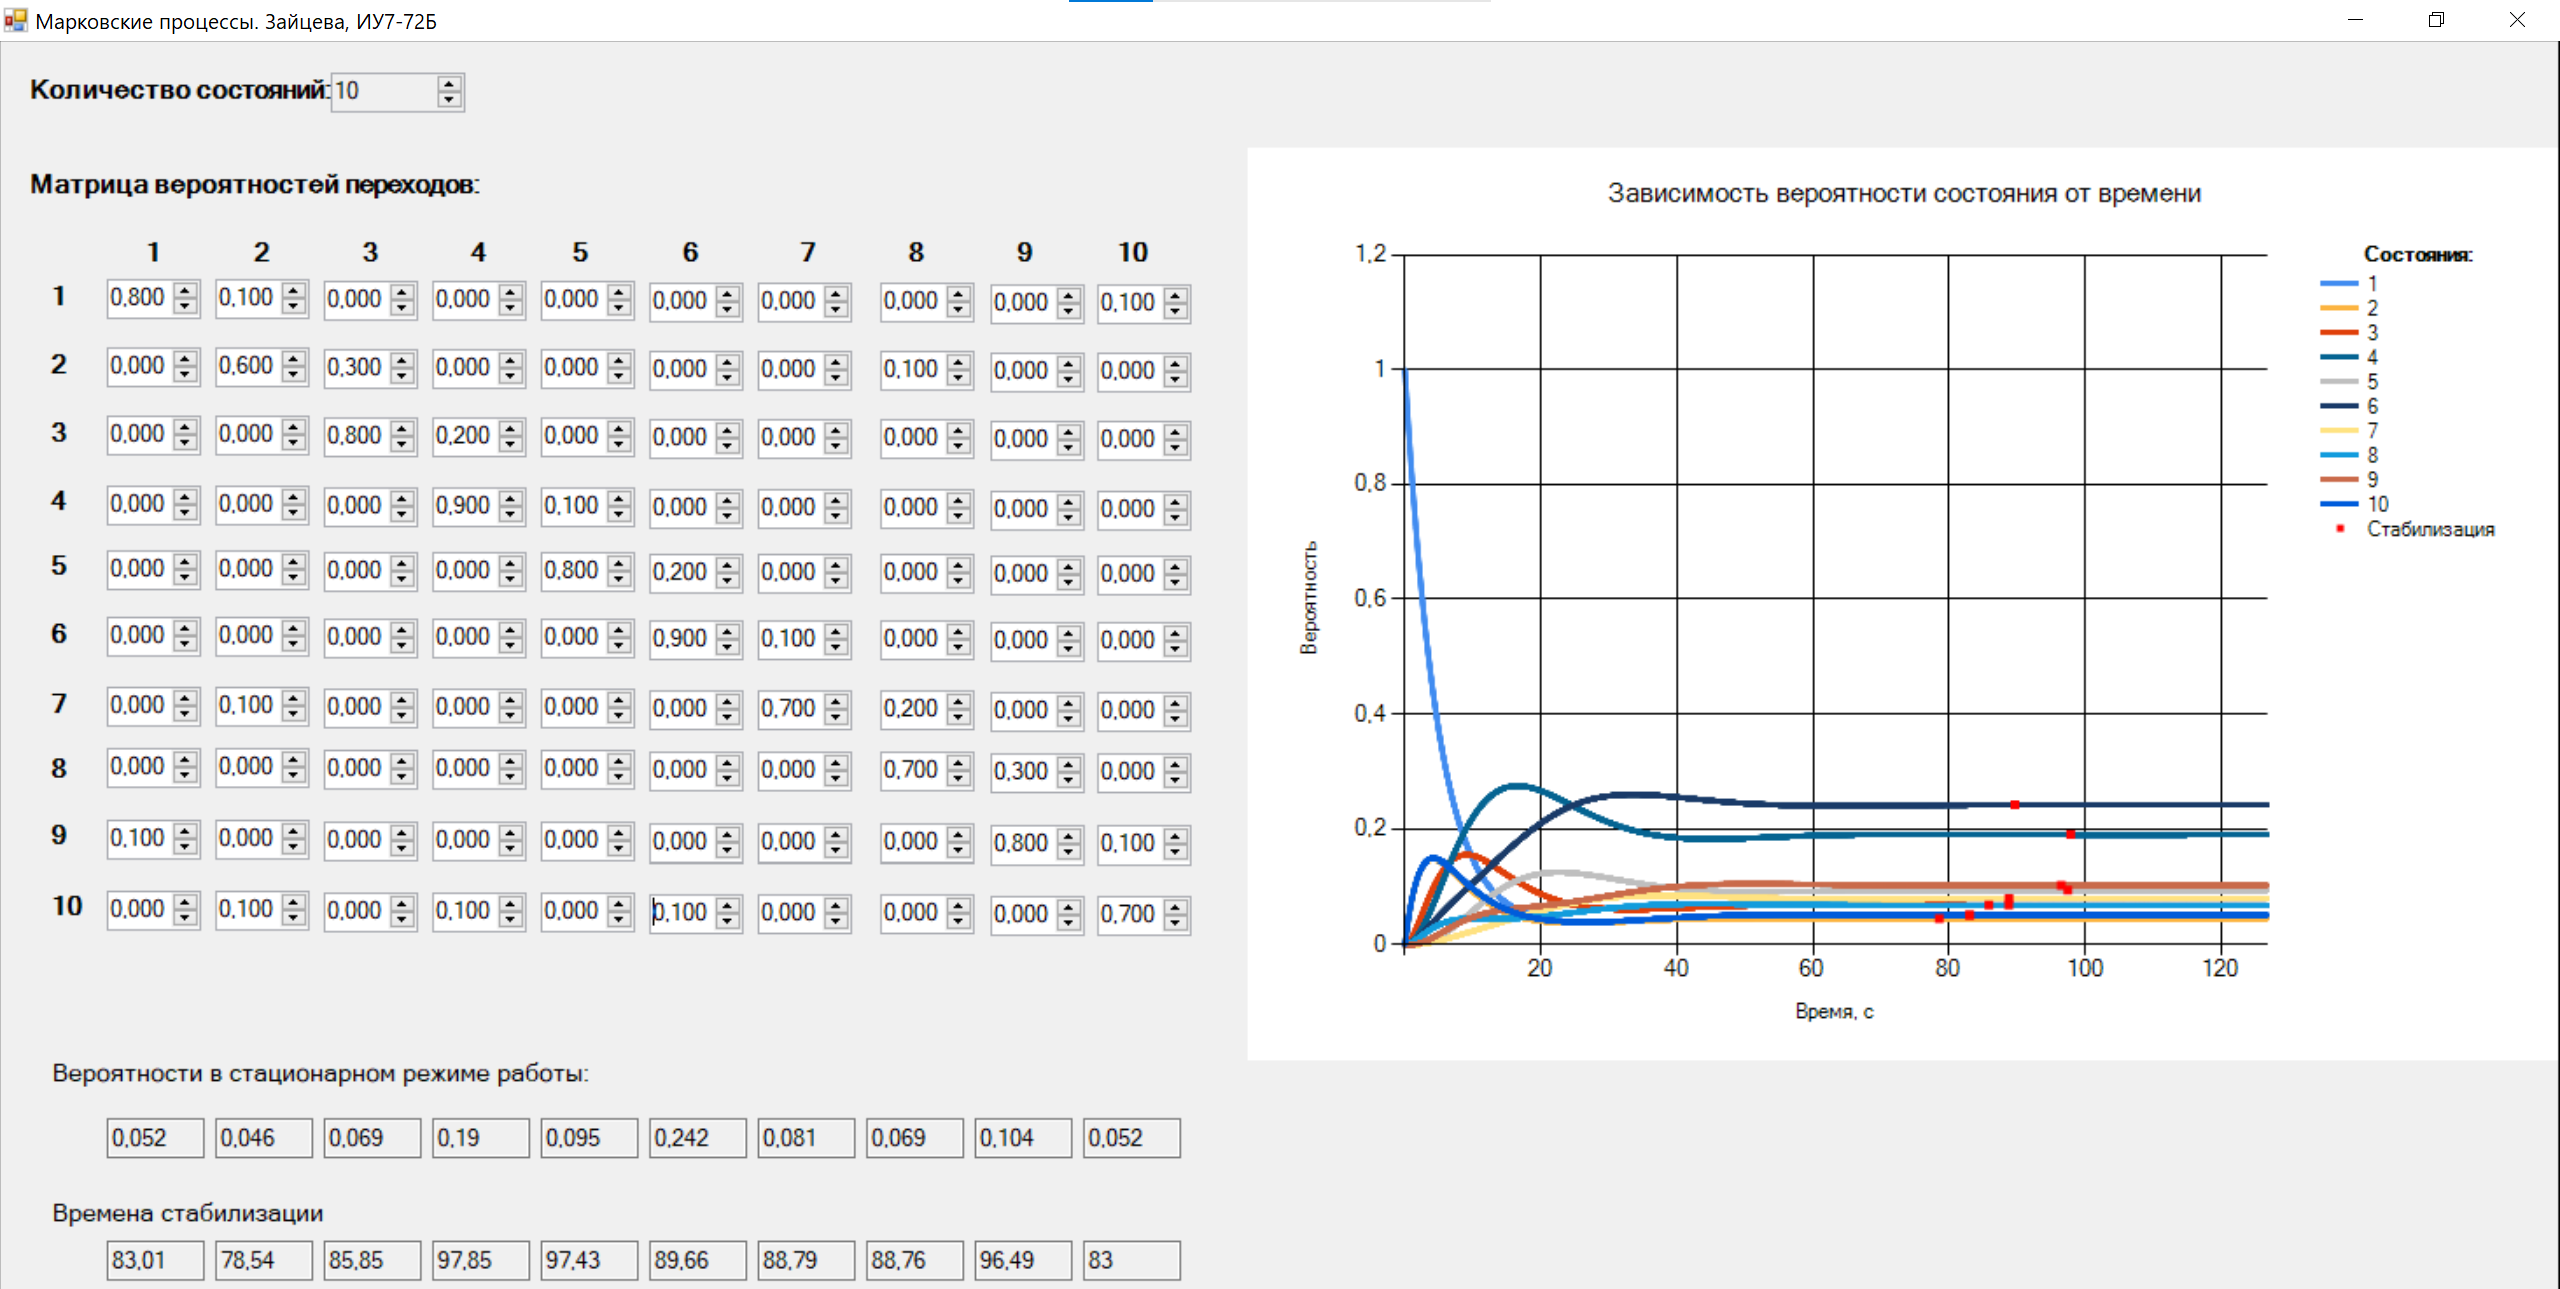
\includegraphics[scale=0.45]{pictures/4.png}
			\caption{Пример работы программы для 10 состояний}
			\label{pic:4}}
	\end{center}
\end{figure}



\section{Код программы}

Класс EmulationModel, используемый для расчетов и построения графиков, приведен в листинге \ref{lst:list1} (используемый язык -- C\#).

\begin{lstlisting}[caption = {Класс EmulationModel, используемый для расчетов и построения графиков}, label=lst:list1]
    class EmulationModel
{
	public int NStates;
	public double[,] mtr;
	public double[] pArr;
	public double[] tStableArr;
	public Chart currentChart;
	readonly double step = 0.01;
	readonly double stabEpsilon = 1e-5;
	readonly double zeroEpsilon = 1e-8;
	
	public EmulationModel(int nStates, ref Chart chart)
	{
		NStates = nStates; 
		pArr = new double[NStates];
		tStableArr = new double[NStates];
		mtr = new double[NStates, NStates];
		currentChart = chart;
		_initParray();
	}
	
	public void Emulate()
	{
		_initSeries();
		double[] deltaProbArray = new double[NStates];
		deltaProbArray[0] = 2 * stabEpsilon;
		
		for (double currentT = step; !_checkModelStabelized(deltaProbArray); currentT += step)
		{
			_drawArrayOnCurrentT(currentT, pArr);
			
			deltaProbArray = new double[NStates];
			double[] PderivativeArr = new double[NStates];
			
			for (int i = 0; i < NStates; i++)
			{
				for (int j = 0; j < NStates; j++)
				{
					double probDensityToAdd = mtr[j, i] * pArr[j] - mtr[i, j] * pArr[i];
					PderivativeArr[i] += probDensityToAdd;
					deltaProbArray[i] += probDensityToAdd * step;
				}
				pArr[i] += deltaProbArray[i];
			}
			
			_checkSomeStatesStabelized(currentT, PderivativeArr);
		}
		_drawStabelizedParr();
	}
	
	private void _initParray()
	{
		pArr[0] = 1;
		for (int i = 1; i < NStates; i++)
		pArr[i] = 0;
	}
	
	private void _initSeries()
	{
		currentChart.Series.Clear();
		for (int i = 0; i < NStates; i++)
		{
			currentChart.Series.Add((i + 1).ToString());
			currentChart.Series[i].ChartType = SeriesChartType.Line;
			currentChart.Series[i].BorderWidth = 3;
		}
		
		currentChart.Series.Add("Стабилизация");
		currentChart.Series[NStates].ChartType = SeriesChartType.Point;
		currentChart.Series[NStates].Color = Color.Red;
	}
	
	private bool _checkModelStabelized(double[] arr)
	{
		for (int i = 0; i < arr.Length; i++)
		if (arr[i] > zeroEpsilon)
		return false;
		return true;
	}
	
	private void _checkSomeStatesStabelized(double currentT, double[] klmArr)
	{
		for (int i = 0; i < NStates; i++)
		{
			if (Math.Abs(klmArr[i]) < stabEpsilon && tStableArr[i] == 0)
			tStableArr[i] = currentT;
			
			else if (Math.Abs(klmArr[i]) > stabEpsilon && tStableArr[i] != 0)
			tStableArr[i] = 0;
		}
	}
	
	private void _drawArrayOnCurrentT(double currentT, double[] arr)
	{
		for (int i = 0; i < NStates; i++)
		{
			currentChart.Series[i].Points.AddXY(currentT, arr[i]);
		}
	}
	
	private void _drawStabelizedParr()
	{
		for (int i = 0; i < NStates; i++)
		{
			currentChart.Series[NStates].Points.AddXY(tStableArr[i], pArr[i]);
		}
	}
}
\end{lstlisting}

\end{document}